\documentclass[11pt,a4paper]{article}

% ---------------------------------------------------------------------------
% Reaction-minimal cusps in planar bimolecular mass-action networks:
% an exhaustive certified classification.
%
% Author metadata: set the three macros below before submission.
% They are deliberately left blank in this version.
% ---------------------------------------------------------------------------
\newcommand{\PaperAuthor}{}
\newcommand{\PaperAffiliation}{}
\newcommand{\PaperDate}{14 September 2026}

\usepackage[T1]{fontenc}
\usepackage[utf8]{inputenc}
\usepackage{lmodern}
\usepackage{microtype}
\usepackage[a4paper,margin=1.05in]{geometry}
\usepackage{amsmath,amssymb,amsthm,mathtools}
\usepackage{booktabs}
\usepackage{array}
\usepackage{longtable}
\usepackage{enumitem}
\usepackage{xcolor}
\usepackage{graphicx}
\usepackage{listings}
\usepackage[obeyspaces,spaces]{url}
\usepackage[numbers,sort&compress]{natbib}
\usepackage[colorlinks=true,linkcolor=blue!55!black,citecolor=blue!55!black,urlcolor=blue!55!black]{hyperref}
\hypersetup{pdftitle={Reaction-minimal cusps in planar bimolecular mass-action networks: an exhaustive certified classification},
  pdfkeywords={mass action, cusp bifurcation, bimolecular reaction network, bistability, Lean, exact certificates, classification}}

\DeclareUrlCommand\lean{\urlstyle{tt}}
\setlist{itemsep=2pt,topsep=3pt}
\setlength{\emergencystretch}{1.5em}
\graphicspath{{figures/}}
\clubpenalty=10000
\widowpenalty=10000

\lstdefinelanguage{Lean}{
  morekeywords={theorem,def,structure,inductive,namespace,end,import,by,intro,exact,constructor,refine,where,abbrev,noncomputable},
  sensitive=true,
  morecomment=[l]{--},
  morestring=[b]",
}
\lstset{
  language=Lean,
  basicstyle=\ttfamily\small,
  keywordstyle=\bfseries,
  commentstyle=\itshape\color{black!60},
  columns=fullflexible,
  keepspaces=true,
  breaklines=true,
  frame=single,
  framerule=0.3pt,
  xleftmargin=1em,
  xrightmargin=1em,
  extendedchars=true,
  literate={≤}{{$\le$}}1 {≥}{{$\ge$}}1 {ℕ}{{$\mathbb{N}$}}1 {ℝ}{{$\mathbb{R}$}}1 {ℤ}{{$\mathbb{Z}$}}1 {→}{{$\to$}}1 {∀}{{$\forall$}}1 {∃}{{$\exists$}}1 {≠}{{$\neq$}}1 {∧}{{$\wedge$}}1 {¬}{{$\neg$}}1 {↔}{{$\leftrightarrow$}}1 {∑}{{$\sum$}}1 {∏}{{$\prod$}}1 {₀}{{$_0$}}1 {₁}{{$_1$}}1 {₂}{{$_2$}}1 {⟨}{{$\langle$}}1 {⟩}{{$\rangle$}}1 {∈}{{$\in$}}1 {λ}{{$\lambda$}}1 {·}{{$\cdot$}}1
}

\theoremstyle{plain}
\newtheorem{theorem}{Theorem}[section]
\newtheorem{proposition}[theorem]{Proposition}
\newtheorem{lemma}[theorem]{Lemma}
\newtheorem{corollary}[theorem]{Corollary}
\theoremstyle{definition}
\newtheorem{definition}[theorem]{Definition}
\newtheorem{example}[theorem]{Example}
\theoremstyle{remark}
\newtheorem{remark}[theorem]{Remark}

\numberwithin{equation}{section}

\newcommand{\R}{\mathbb{R}}
\newcommand{\Q}{\mathbb{Q}}
\newcommand{\N}{\mathbb{N}}
\newcommand{\Z}{\mathbb{Z}}
\newcommand{\T}{\mathsf{T}}
\newcommand{\one}{\mathbf{1}}
\newcommand{\Diag}{\operatorname{diag}}
\newcommand{\rank}{\operatorname{rank}}
\newcommand{\tr}{\operatorname{tr}}
\newcommand{\im}{\operatorname{im}}
\newcommand{\Ker}{\operatorname{ker}}
\newcommand{\Class}{\mathcal{C}}
\newcommand{\Eligible}{\mathcal{E}}
\newcommand{\AlgCusp}{\mathsf{AlgCusp}}

\title{Reaction-minimal cusps in planar bimolecular mass-action networks: an exhaustive certified classification}
\author{\PaperAuthor\\ \small \PaperAffiliation}
\date{\PaperDate}

\begin{document}
\maketitle

\begin{abstract}
A cusp of equilibria is the simplest generic mechanism by which a two-parameter family of vector fields passes between one and three nearby equilibria, and it organizes bistability in chemical reaction networks. We classify the two-species, five-reaction, rank-two bimolecular mass-action networks that admit a positive nondegenerate cusp transversely unfolded by two independent rate constants. Up to reaction permutation, positive rescaling of stoichiometric columns with reactants fixed, and exchange of the two species, there are exactly 52 such networks, and every one of them uses five distinct reactant complexes. Combined with the four-reaction exclusion of Banaji, Boros and Hofbauer, five reactions is the minimum reaction count for a rate-transverse cusp in planar bimolecular mass-action kinetics. The proof is exhaustive and certified. Necessary structural conditions reduce the $142{,}506$ literal five-reaction sets to $60{,}036$ eligible ones, and a reactant-labelled primitive-ray key collapses these to $9{,}999$ mechanism classes. Every class is decided by an exact rational certificate: $9{,}063$ determinant obstructions, $744$ quadratic-degeneracy obstructions, $140$ cubic-degeneracy obstructions and $52$ positive templates. The algebraic classification, including source-faithful coverage of every eligible literal network, is an unconditional theorem verified in Lean~4 against Mathlib. The passage to ordinary analytic cusps is a Lyapunov--Schmidt reduction of the planar vector field that makes explicit a correction to the parameter-unfolding derivative missing from the formal predicate; the corrected minors of all 52 templates are certified by exact rational-polynomial B\'ezout identities. Every one of the 52 classes organizes nearby positive stable--saddle--stable triples, and we exhibit a fully rational template whose equilibrium equation reduces exactly to $\mu+\nu z-z^{3}$. The paper separates the Lean-verified core from the conventional arguments and exact computer-algebra checks, records the native-evaluation trust boundary, and lists all 52 representatives.
\end{abstract}

\section{Introduction}\label{sec:intro}

\subsection{Cusps and minimal networks}
Under mass-action kinetics, a chemical reaction network with $n$ species and $m$ reactions defines a polynomial vector field on the positive orthant, parameterized by $m$ positive rate constants. Which qualitative behaviours a network can display, and how few reactions are needed to display them, are classical questions of chemical reaction network theory~\citep{Feinberg2019}. For multiple positive equilibria the questions have precise answers in several settings: injectivity criteria exclude multistationarity in large classes of networks~\citep{CF2005}, parameter regions for multistationarity can be described algebraically~\citep{CFMW2017}, and the smallest networks with multiple or bistable equilibria have been enumerated in specific model classes~\citep{Wilhelm2009,JS2013}. Inheritance results explain why small networks matter: a nondegenerate behaviour of a subnetwork is passed to any enlargement obtained by a list of admissible operations, so the small networks are the atoms from which the behaviour of larger networks can be read off~\citep{BP2018,BBH2022,BBH2025}.

The bifurcation that organizes bistability is the cusp. At a cusp of equilibria a two-parameter family of vector fields has a fold curve with a cusp point, and inside the cusp region an equilibrium with a simple zero eigenvalue has split into three nearby equilibria~\citep{Kuznetsov2004,GS1985}. For mass-action systems the relevant question is whether a cusp can occur at positive concentrations and be unfolded transversely by the rate constants themselves, since the rate constants are the only parameters the network provides. Banaji, Boros and Hofbauer classified local bifurcations in planar quadratic mass-action networks with few reactions and, in particular, proved that no full-rank planar network with four reactions admits a cusp unfolded by its rates~\citep{BBH2024}; earlier, Banaji and Boros determined the smallest bimolecular networks admitting Andronov--Hopf bifurcation~\citep{BB2023}, and three-reaction quadratic networks with oscillations were analysed in~\citep{BBH2024osc}. Five reactions is therefore the first count at which a planar bimolecular cusp can occur.

\subsection{The result}
We give an exhaustive certified classification of the five-reaction case. The model is the set of networks with two species, five distinct directed reactions between the six bimolecular complexes $0,X,Y,2X,X+Y,2Y$, no self-reactions, stoichiometric rank two, and independent positive rate constants. The equivalence is the natural one under which the family of vector fields is preserved: reaction permutation, positive rescaling of each stoichiometric column with its reactant fixed (which is an invertible reparameterization of the rates), and exchange of the two species. The main theorem (Theorem~\ref{thm:main}) states that a network in the model admits a positive nondegenerate cusp transversely unfolded by two of its rate constants if and only if its class is one of 52 listed classes. Every one of these classes has five distinct reactant complexes (Corollary~\ref{cor:five-sources}), and five reactions is minimal (Corollary~\ref{cor:minimal}). The classification is a count of network classes, not of cusp points or parameter regions.

The proof is a decision procedure with certificates. Necessary conditions from the equilibrium and jet equations cut the $\binom{30}{5}=142{,}506$ literal reaction sets down to $60{,}036$ eligible ones; a reactant-labelled primitive-ray key that is a complete invariant of the equivalence (Lemma~\ref{lem:key}) reduces these to $9{,}999$ mechanism classes. Each class is decided by one of three exact rational obstruction schemes or by an exact positive template. The obstruction schemes are sound for every positive equilibrium flux of the network, not for sampled rate values: a determinant certificate proves that the Jacobian cannot be singular at any positive equilibrium, a quadratic-degeneracy certificate proves that a singular Jacobian cannot have vanishing quadratic center coefficient, and a cubic-degeneracy certificate proves that the required center equations force the cubic coefficient to vanish. A positive template supplies an exact algebraic equilibrium, rates and jet vectors, with a root polynomial and a rational isolating interval.

\subsection{Two levels of verification}
The classification has two complementary verification levels, and we keep them distinct throughout.

The \emph{formal core} is an unconditional theorem verified in Lean~4~\citep{Lean4} against Mathlib~\citep{mathlib2020}: for every literal network $Q$ in the model, an algebraic cusp certificate for $Q$ exists if and only if $Q$ is source-faithfully covered by one of the 52 positive classes. The algebraic certificate is the jet system of Section~\ref{sec:cusp} together with a raw two-parameter rank condition. The formal theorem quantifies over the literal networks, not over a hand-chosen list of representatives, and its coverage step proves that each of the $60{,}036$ eligible literal reaction sets is connected by an explicit equivalence to the actual stored record that classifies it. This is the part of the proof for which a machine check is most valuable: it is a large finite case analysis whose correctness depends on exact bookkeeping.

The \emph{analytic interpretation} is a conventional local reduction. The formal predicate's parameter row is the raw derivative $pJ_k(u)q$, whereas the Lyapunov--Schmidt reduction of the vector field produces the corrected row $pJ_k(u)q-pB(q,f_k(u))/\tau$. We prove that every ordinary transverse cusp in the model satisfies the formal predicate (Lemma~\ref{lem:necessary}), so the formal negative direction excludes ordinary cusps, and we verify the corrected minor for each of the 52 positive templates by an exact B\'ezout identity in $\Q[t]$ (Proposition~\ref{prop:positive}). The analytic reduction and the 52 corrected-minor instances are exact mathematics plus reproducible computer algebra; they are not relabelled as Lean theorems. Section~\ref{sec:verification} tabulates which statements are formal and which are conventional, and records the trust boundary of the formal part, which uses Lean's compiled native evaluation for finite computations.

\subsection{Related and concurrent work}
Banaji and Feliu's bounds on positive equilibria in terms of the number of distinct sources~\citep{BF2026} give an independent explanation of one of our structural reductions: a full-rank planar network with at most three sources cannot produce the three nearby isolated positive equilibria that a transverse cusp requires. Banaji's preprint of 7~September 2026~\citep{B2026} establishes a correspondence between fold and cusp conditions for the original and dual equations of a mass-action system, and its Section~6.3 announces a forthcoming classification of the same $(2,5,2)$ bimolecular class. We make no priority claim and do not claim agreement with a representative list that has not been compared. Our analytic conditions are derived directly from the planar vector field, and our verification levels are stated so that any future comparison can be made class by class using the keys of Appendix~\ref{app:list}. Large certificate-based formal classifications have precedents in the formal proofs of the four-colour theorem~\citep{Gonthier2008} and the Kepler conjecture~\citep{Hales2017}; the proof-engineering point of the present work is the separation of compact keys from large algebraic payloads in the coverage step (Section~\ref{sec:coverage}).

\subsection{Organization}
Section~\ref{sec:model} fixes the model and the equivalence, and states the main theorem and its corollaries. Section~\ref{sec:cusp} derives the local cusp criterion and relates it to the formal predicate. Section~\ref{sec:reductions} proves the structural reductions and describes the finite enumeration. Section~\ref{sec:negative} presents the three obstruction schemes and their soundness. Section~\ref{sec:positive} presents the positive templates and a fully rational example. Section~\ref{sec:coverage} describes the formal coverage theorem and proves the main theorem. Section~\ref{sec:consequences} derives consequences: five sources are necessary, every class organizes bistability, ray geometry alone does not decide cusp existence, and cusps are inherited by admissible enlargements. Section~\ref{sec:verification} records the verification and reproducibility data, and Section~\ref{sec:discussion} lists open problems. Appendix~\ref{app:list} contains the complete list of 52 representatives.

\section{Networks, equivalence and the main theorem}\label{sec:model}

\subsection{The model}
Let
\[
 \Class=\{(0,0),(1,0),(0,1),(2,0),(1,1),(0,2)\}=\{0,X,Y,2X,X+Y,2Y\}
\]
be the six complexes of molecularity at most two in two species. A \emph{network} is a set of five distinct ordered pairs $a_r\to b_r$ with $a_r,b_r\in\Class$ and $a_r\ne b_r$. Reactions are indexed by $r=1,\dots,5$ only to write formulas; the index order is immaterial. Set
\[
 N_r=b_r-a_r\in\Z^2,\qquad N=(N_1\ \cdots\ N_5)\in\Z^{2\times5},\qquad
 A=\begin{pmatrix}a_1^{\T}\\ \vdots\\ a_5^{\T}\end{pmatrix}\in\Z^{5\times2}.
\]
We require $\rank N=2$; in particular both species occur in some reaction. With rate constants $k=(k_1,\dots,k_5)$, $k_r>0$, the mass-action system is
\begin{equation}\label{eq:mass}
 \dot x=f(x,k)=\sum_{r=1}^5 N_r\,k_r\,x^{a_r},\qquad x^{a_r}=x_1^{a_{r1}}x_2^{a_{r2}},\qquad x\in\R^2_{>0}.
\end{equation}
Since every complex is bimolecular, $f$ is a quadratic polynomial in $x$ and linear in $k$. Self-reactions and duplicate directed reactions are excluded, but distinct reactions may share a reactant, and no relation between rate constants and no conservation law is imposed.

The four defining conditions (reactant and product molecularity at most two, rank two, both species used) are exactly the hypotheses of the formal predicate \lean{IsPlanarBimolecular252} in the Lean development, and the five-reaction structure with distinct reactions and no self-reactions is the type \lean{SmallPlanarNetwork 5} (Section~\ref{sec:coverage}).

\subsection{Equivalence}
\begin{definition}\label{def:equiv}
Two networks are \emph{simply equivalent up to species exchange} if, after permuting reactions and optionally exchanging the two species, their reactants agree reaction by reaction and their stoichiometric columns satisfy $N'_r=\lambda_rN_r$ for some $\lambda_r>0$.
\end{definition}

The substitution $k'_r=k_r/\lambda_r$ identifies the families of vector fields of two simply equivalent networks, and species exchange is a linear change of state coordinates. Every property considered in this paper is therefore invariant under Definition~\ref{def:equiv}. We do not quotient by anything larger: not by arbitrary dynamical equivalence, not by diagonal row rescaling of $N$, and not by general changes of state coordinates. The count below is a count of classes under Definition~\ref{def:equiv}.

For a nonzero integer vector $v$ let $\bar v=v/\gcd(|v_1|,|v_2|)$ be its primitive vector; the denominator is positive, so $v$ and $-v$ have distinct primitive vectors. Define the \emph{key} $K(Q)$ of a network $Q$ as the lexicographically smaller of the two sorted multisets
\begin{equation}\label{eq:key}
 \{\!\{(a_r,\bar N_r):1\le r\le5\}\!\}\qquad\text{and its species-exchanged copy.}
\end{equation}

\begin{lemma}\label{lem:key}
Two networks in the model have equal keys if and only if they are equivalent in the sense of Definition~\ref{def:equiv}.
\end{lemma}
\begin{proof}
Positive column scaling fixes the reactant and the primitive directed vector of each reaction, reaction permutation fixes the multiset, and species exchange sends each multiset to its exchanged copy; hence equivalent networks have equal keys. Conversely, equality of the sorted multisets, after at most one species exchange, matches the reactions one by one with equal reactants and equal primitive vectors. Each integer column is a positive integer multiple of its primitive vector, so the ratio of the two multiples is the required $\lambda_r>0$. Multiplicities are part of the multiset, so repeated labelled rays are matched correctly.
\end{proof}

\subsection{The main theorem}
Here and below an \emph{ordinary transverse cusp} of a network is a nondegenerate cusp of equilibria of the smooth family~\eqref{eq:mass} at a positive state $x^*$ and positive rates $k^*$: the Jacobian has a simple zero eigenvalue with nonzero complementary eigenvalue, the reduced equilibrium equation has a zero of order exactly three, and two of the rate constants unfold it regularly. Section~\ref{sec:cusp} gives the precise local test.

\begin{theorem}[Classification]\label{thm:main}
For a network $Q$ in the model, the following are equivalent.
\begin{enumerate}[label=\textup{(\roman*)}]
\item $Q$ admits an ordinary transverse cusp at positive concentrations and positive rate constants.
\item $K(Q)$ is one of the 52 keys represented by the rows of Table~\ref{tab:all} in Appendix~\ref{app:list}.
\end{enumerate}
The 52 representatives are pairwise inequivalent under Definition~\ref{def:equiv}.
\end{theorem}

\begin{corollary}[Five sources are necessary]\label{cor:five-sources}
Every network in the model that admits an ordinary transverse cusp has five distinct reactant complexes. Networks with four distinct reactants, which form $8{,}000$ of the $9{,}999$ mechanism classes and satisfy the general lower bound of four sources, never admit one.
\end{corollary}

\begin{corollary}[Reaction minimality]\label{cor:minimal}
Five reactions is the minimum number of reactions for which a planar bimolecular mass-action network admits a cusp transversely unfolded by its rate constants, and each of the 52 classes attains it.
\end{corollary}

\begin{corollary}[Bistability]\label{cor:bistable}
Every one of the 52 classes admits positive rate constants at which the system has three positive equilibria, two of which are asymptotically stable and one a saddle, all three in a neighbourhood of a cusp point.
\end{corollary}

The corollaries are proved in Section~\ref{sec:consequences}. Theorem~\ref{thm:main} is proved in Section~\ref{sec:coverage} after the ingredients have been assembled: the local criterion (Section~\ref{sec:cusp}), the structural reductions (Section~\ref{sec:reductions}), the soundness of the three obstruction schemes (Section~\ref{sec:negative}), the positive templates (Section~\ref{sec:positive}) and the formal coverage theorem (Section~\ref{sec:coverage}).

\section{The planar quadratic cusp criterion}\label{sec:cusp}

All derivatives in this section are evaluated at a positive equilibrium $(x^*,k^*)$ of~\eqref{eq:mass}. Write $J=f_x$ for the Jacobian and $B=f_{xx}$ for the symmetric bilinear second derivative without a factorial factor, so that $f(x^*+\xi,k^*)=J\xi+\tfrac12B(\xi,\xi)$ exactly, because $f$ is quadratic in $x$. Write $f_k(u)$ and $J_k(u)$ for the derivatives of $f$ and $J$ in the rate direction $u\in\R^5$; both are linear in $u$ because $f$ is linear in $k$.

\subsection{The jet system}
Suppose that
\begin{equation}\label{eq:jet}
 \begin{gathered}
 Jq=0,\qquad pJ=0,\qquad pq=1,\qquad \tau=\tr J\ne0,\\
 pB(q,q)=0,\qquad Jh=-B(q,q),\qquad ph=0,
 \end{gathered}
\end{equation}
where $p$ is a row vector and $q,h$ are column vectors. The first line says that $0$ is a simple eigenvalue of $J$ with complementary eigenvalue $\tau$; then $P=I-qp$ is the spectral projection onto $\im J=\Ker p$ and $J=\tau P$. Consequently the center-correction equation $Jh=-B(q,q)$ has a solution precisely when $pB(q,q)=0$, and then a unique solution with $ph=0$. The second line says that the quadratic coefficient of the reduced equation vanishes and fixes the center correction.

For a rate direction $u\in\R^5$ define
\begin{equation}\label{eq:rows}
 a(u)=p\,f_k(u),\qquad
 b(u)=p\,J_k(u)\,q-\frac{p\,B(q,f_k(u))}{\tau},\qquad
 c=\tfrac12\,p\,B(q,h).
\end{equation}

\begin{proposition}[Local analytic test]\label{prop:analytic}
Assume~\eqref{eq:jet}. The equilibrium $(x^*,k^*)$ is a nondegenerate cusp of equilibria of~\eqref{eq:mass} transversely unfolded by the rate constants $k_i,k_j$ if and only if $c\ne0$ and
\begin{equation}\label{eq:corrected}
 \det\begin{pmatrix}a(e_i)&a(e_j)\\ b(e_i)&b(e_j)\end{pmatrix}\ne0,
\end{equation}
where $e_i,e_j$ are the coordinate directions in rate space. The equilibrium is a cusp transversely unfolded by \emph{some} pair of rates if and only if $c\ne0$ and the $2\times5$ matrix with rows $a$ and $b$ has rank two.
\end{proposition}

\begin{proof}
Resolve nearby states as $x=x^*+zq+y$ with $y\in\Ker p$, so that $z=p(x-x^*)$. The transverse component $Pf(x^*+zq+y,k)=0$ of the equilibrium equation is an equation in $\Ker p$ whose derivative in $y$ at the base point is $J|_{\Ker p}=\tau\,\mathrm{id}$, which is invertible. By the implicit function theorem it has a unique smooth local solution $y=y(z,k)$ with $y(0,k^*)=0$, and equilibria of~\eqref{eq:mass} near $(x^*,k^*)$ correspond exactly to the zeros of the reduced scalar function
\[
 g(z,k)=p\,f\bigl(x^*+zq+y(z,k),k\bigr).
\]
This is the Lyapunov--Schmidt reduction~\citep[Chapter~I]{GS1985}. Implicit differentiation at the base point gives
\[
 y_z=0,\qquad y_{zz}=h,\qquad y_k(u)=-\frac{Pf_k(u)}{\tau}.
\]
Indeed $\tau y_z=-PJq=0$; $\tau y_{zz}=-PB(q,q)=-B(q,q)$ because $pB(q,q)=0$, and $y_{zz}\in\Ker p$ identifies it with $h$; and $\tau y_k(u)=-Pf_k(u)$. Differentiating $g$, and using that $f$ has no third derivative in $x$,
\[
 g=g_z=g_{zz}=0,\qquad g_{zzz}=3\,pB(q,y_{zz})=3\,pB(q,h)=6c,
\]
and
\[
 \begin{aligned}
 g_k(u)&=p\,f_k(u)=a(u),\\
 g_{zk}(u)&=p\,J_k(u)\,q+p\,B(q,y_k(u))=p\,J_k(u)\,q-\frac{pB(q,f_k(u))}{\tau}=b(u),
 \end{aligned}
\]
where the last step expands $pB(q,y_k(u))=-\tau^{-1}\bigl(pB(q,f_k(u))-pB(q,q)\,pf_k(u)\bigr)$ and uses $pB(q,q)=0$. A scalar equation $g(z,\mu)=0$ with $g=g_z=g_{zz}=0$ and $g_{zzz}\ne0$ at the origin has a versal two-parameter unfolding by $(k_i,k_j)$ exactly when the map $(k_i,k_j)\mapsto(g,g_z)$ has invertible derivative, which is~\eqref{eq:corrected}~\citep[Chapter~III, the cusp or hysteresis normal form $z^3$]{GS1985}. Because the complementary eigenvalue $\tau$ is nonzero, the zero set of $g$ is the full local equilibrium set of the vector field, and these are the defining conditions of a nondegenerate cusp bifurcation of equilibria~\citep[Section~8.2]{Kuznetsov2004}. The last assertion follows because the pairs of columns of the $2\times5$ matrix $(a;b)$ span it if and only if it has rank two.
\end{proof}

\begin{remark}[Conventions]\label{rem:conventions}
The normalization $pq=1$ suffices; no Euclidean unit convention on $q$ is needed. Replacing $q$ by $\alpha q$ with $\alpha\ne0$ forces $p\mapsto p/\alpha$ and $h\mapsto\alpha^2h$, so $c\mapsto\alpha^2c$: the vanishing and the sign of $c$ are independent of the normalization. The sign of $c$ enters only in Corollary~\ref{cor:bistable}. In the convention of~\citep{B2026} the center correction solves $Jh_{\mathrm B}=B(q,q)$, so $h_{\mathrm B}=-h$ and the cubic condition is the same. Table~\ref{tab:dictionary} records the correspondence with the standard cusp conditions.
\end{remark}

\begin{table}[tb]
\centering\small
\caption{The standard equilibrium-cusp conditions of a planar vector field and their exact specialization to the quadratic mass-action system~\eqref{eq:mass}. The labels B1, B2, B4, B5 follow~\citep{B2026}.}
\label{tab:dictionary}
\begin{tabular}{p{.42\linewidth}p{.50\linewidth}}\toprule
Standard condition & Exact specialization\\\midrule
B1: simple zero eigenvalue, no other eigenvalue on the imaginary axis & $\det J=0$, $\tau=\tr J\ne0$; then $J=\tau(I-qp)$\\
B2: vanishing quadratic coefficient of the reduced equation & $pB(q,q)=0$\\
Center correction & $Jh=-B(q,q)$, $ph=0$\\
B4: nonvanishing cubic coefficient & $c=\tfrac12pB(q,h)\ne0$\\
B5: two-parameter transversality by rates $k_i,k_j$ & $\det$ of the columns $i,j$ of the rows $u\mapsto pf_k(u)$ and $u\mapsto pJ_k(u)q-pB(q,f_k(u))/\tau$ is nonzero\\\bottomrule
\end{tabular}
\end{table}

\subsection{The formal predicate and why it is necessary}
The correction term in $b(u)$ is essential, and it is the point at which the formal and analytic levels of the paper differ. The Lean predicate used by the algebraic classification asks for an exact certificate consisting of a positive state, positive rates, vectors $p,q,h$ and two rate directions $u^1,u^2$ such that the equilibrium equation holds, all of~\eqref{eq:jet} holds, $pB(q,h)\ne0$, and the \emph{raw} $2\times2$ matrix
\begin{equation}\label{eq:raw}
 \begin{pmatrix} p\,f_k(u^1) & p\,f_k(u^2)\\ p\,J_k(u^1)\,q & p\,J_k(u^2)\,q\end{pmatrix}
\end{equation}
has nonzero determinant. We denote this existential predicate by $\AlgCusp(Q)$; it is the predicate \lean{AdmitsTransverseCusp} of Section~\ref{sec:coverage}. Nonvanishing of~\eqref{eq:raw} for some pair of directions is equivalent to rank two of the $2\times5$ matrix of raw rows.

\begin{lemma}[Necessary formal certificate]\label{lem:necessary}
Every ordinary transverse cusp of a network in the model satisfies $\AlgCusp(Q)$.
\end{lemma}
\begin{proof}
An ordinary transverse cusp supplies positive $(x^*,k^*)$, the jet system~\eqref{eq:jet}, and $pB(q,h)=2c\ne0$. It remains to produce two rate directions on which the raw matrix~\eqref{eq:raw} is nonsingular. Define
\[
 u_r=k^*_r\sum_{\ell=1}^2 a_{r\ell}\,\frac{h_\ell}{x^*_\ell}\quad(r=1,\dots,5),\qquad
 w_\ell=\frac{q_\ell h_\ell}{x^*_\ell}\quad(\ell=1,2).
\]
Termwise differentiation of~\eqref{eq:mass} gives the identities
\[
 f_k(u)=Jh,\qquad J_k(u)\,q=B(q,h)+Jw.
\]
The first holds because $\sum_r N_r u_r (x^*)^{a_r}=\sum_r N_rk^*_r(x^*)^{a_r}\sum_\ell a_{r\ell}h_\ell/x^*_\ell=Jh$; the second follows by differentiating the first identity in the state direction. Hence $pf_k(u)=pJh=0$ and $pJ_k(u)q=pB(q,h)\ne0$. Since $\rank N=2$, the row $u\mapsto pf_k(u)=\sum_r pN_r\,(x^*)^{a_r}u_r$ is nonzero: $p\ne0$, the columns $N_r$ span $\R^2$, and every $(x^*)^{a_r}$ is positive. Choose $v$ with $pf_k(v)\ne0$. The raw matrix on $(v,u)$ is lower triangular with nonzero diagonal, so its determinant $pf_k(v)\cdot pB(q,h)$ is nonzero. Both directions are admissible because the base rates lie in the interior of the positive orthant.
\end{proof}

We use only this direction of the relationship. The converse is false in general: the raw rank condition does not imply the corrected condition~\eqref{eq:corrected}. For the positive direction of Theorem~\ref{thm:main} the corrected minors are checked exactly on every positive template (Section~\ref{sec:positive}).

\section{Structural reductions and finite enumeration}\label{sec:reductions}

\subsection{Positive flux balance}
At a positive equilibrium let $v_r=k_r(x^*)^{a_r}>0$ be the reaction fluxes. Then
\begin{equation}\label{eq:flux}
 v>0,\qquad Nv=0,\qquad J=N\,\Diag(v)\,A\,\Diag(1/x^*).
\end{equation}

\begin{lemma}\label{lem:surround}
Let $N\in\Z^{2\times5}$ have rank two. There is a strictly positive $v$ with $Nv=0$ if and only if for every column $N_r$ some column has positive cross product with $N_r$ and some column has negative cross product with $N_r$.
\end{lemma}
\begin{proof}
If $Nv=0$ with $v>0$, take the cross product of both sides with $N_r$: a sum $\sum_s v_s\,(N_r\times N_s)$ with strictly positive weights vanishes, and rank two ensures that at least one term is nonzero, so both signs occur. Conversely, the condition says that no closed half-plane bounded by a line through the origin contains all columns; since the columns span the plane, the origin then lies in the interior of their convex hull, which is equivalent to a strictly positive balancing vector.
\end{proof}

\subsection{At least four distinct reactants}
\begin{lemma}\label{lem:four}
A network in the model that admits an ordinary transverse cusp has at least four distinct reactant complexes.
\end{lemma}
\begin{proof}
Inside the cusp region of the unfolding of Proposition~\ref{prop:analytic}, the reduced equation has three simple zeros, so for suitable positive rates arbitrarily close to $k^*$ the system has three isolated positive equilibria. By the few-source bound of Banaji and Feliu~\citep[Corollary~4.25]{BF2026}, a rank-two planar mass-action network whose reactions have at most three distinct sources cannot have three isolated positive equilibria for any choice of rates.
\end{proof}

The Lean development proves the same conclusion for $\AlgCusp$ by a direct algebraic argument that does not use~\citep{BF2026}: after grouping reactions by equal reactants, the vector field has at most three monomials, and for each of four kernel charts covering the possible nonzero singular Jacobians the mixed cubic contraction $pB(q,h)$ is forced to vanish by the singular-equilibrium equations. The two arguments are independent; either suffices for the classification.

\subsection{The eligible catalogue}
There are 30 directed non-self reactions on $\Class$, hence $\binom{30}{5}=142{,}506$ literal five-reaction sets. Call a set \emph{eligible} if it satisfies rank two, the surrounding condition of Lemma~\ref{lem:surround}, and at least four distinct reactants. By~\eqref{eq:flux}, Lemma~\ref{lem:surround} and Lemma~\ref{lem:four}, every cusp-admitting network is eligible. (The Lean enumeration also records affine spanning of the reactants; in the six-point configuration $\Class$ a line contains at most three points, so four distinct reactants already span the plane affinely, and the condition is implied.) The set $\Eligible$ of eligible literal reaction sets has $60{,}036$ elements; its quotient by species exchange has $30{,}051$ elements, and its quotient by the key~\eqref{eq:key} has $9{,}999$ elements (Figure~\ref{fig:coverage}).

\begin{figure}[tb]
\centering
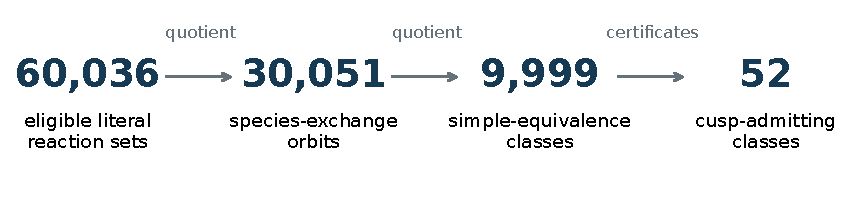
\includegraphics[width=\linewidth]{catalogue_flow.pdf}
\caption{The levels of the classification. The first two arrows are quotients of the eligible literal reaction sets, by species exchange and by the complete invariant of Lemma~\ref{lem:key}; only the last arrow selects the cusp-admitting classes. The formal coverage records retain the exact literal source and its species orientation.}
\label{fig:coverage}
\end{figure}

These counts are exact finite computations. The number $60{,}036$ is a Lean theorem (\lean{structurallyEligibleSourceCatalogue_card}), and the check script accompanying the paper re-enumerates all $142{,}506$ sets independently, applies the three filters, and recovers $60{,}036$, $30{,}051$ and $9{,}999$; it also verifies that the keys of the networks extracted from the four Lean certificate layers are pairwise distinct and exhaust the keys of $\Eligible$.

\subsection{Unit-state normalization}\label{sec:normalization}
The obstruction certificates of Section~\ref{sec:negative} are stated for the polynomial vector field
\[
 F_v(\xi)=\sum_r N_r\,v_r\,\xi^{a_r}\qquad\text{at }\xi=\one,
\]
whose Jacobian and Hessian at $\one$ we denote $J_v=N\Diag(v)A$ and $B_v$. With $D_x=\Diag(x^*)$ these are related to the derivatives of $f$ at $(x^*,k^*)$ by
\[
 J_v=JD_x,\qquad B_v(s,t)=B(D_xs,D_xt).
\]
Hence if $(p,q,h)$ satisfy~\eqref{eq:jet} for $f$, then $q'=D_x^{-1}q$, $h'=D_x^{-1}h$ and $p'=p$ satisfy
\[
 J_vq'=0,\quad p'J_v=0,\quad p'B_v(q',q')=0,\quad J_vh'=-B_v(q',q'),\quad p'B_v(q',h')=pB(q,h)\ne0 .
\]
The normalization preserves the kernel, quadratic-degeneracy, center-correction and nonzero mixed-cubic conditions. It does \emph{not} preserve $p'q'=1$, $p'h'=0$ or the trace, and the obstruction proofs use only the preserved, trace-free conditions. This is recorded because a change of normalization must not silently change the class of singularities being excluded: the negative certificates exclude a singular positive equilibrium with vanishing quadratic and nonvanishing cubic center coefficients, a strictly larger class than the cusps of Proposition~\ref{prop:analytic}.

\section{Three exact obstruction schemes}\label{sec:negative}

All statements in this section concern arbitrary positive unit-equilibrium fluxes $v$ of a fixed network, that is, all $v>0$ with $Nv=0$; nothing is sampled. Let
\[
 d(v)=\det J_v,\qquad J_v=N\Diag(v)A,
\]
a quadratic form in $v$ with integer coefficients. The certificates have rational coefficients, their generic soundness lemmas are Lean theorems, and each instance is checked in Lean by exact rational arithmetic. Table~\ref{tab:counts} gives the numbers of mechanism classes decided by each scheme, split by the number of distinct reactants.

\begin{table}[tb]
\centering
\caption{The exhaustive partition of the $9{,}999$ mechanism classes by the certificate that decides them. The source count is the number of distinct reactant complexes.}
\label{tab:counts}
\begin{tabular}{lrrr}\toprule
Certificate type & Four sources & Five sources & Total\\\midrule
Determinant obstruction & 7,205 & 1,858 & 9,063\\
Quadratic-degeneracy obstruction & 663 & 81 & 744\\
Cubic-degeneracy obstruction & 132 & 8 & 140\\
Positive cusp template & 0 & 52 & 52\\\midrule
Total & 8,000 & 1,999 & 9,999\\\bottomrule
\end{tabular}
\end{table}

\subsection{Determinant obstructions}
A determinant certificate consists of a rational multiplier $\sigma\ne0$ and linear forms $L_1,L_2$ such that
\begin{equation}\label{eq:detcert}
 \sigma\,d(v)-\sum_{\ell=1}^2 L_\ell(v)\,(Nv)_\ell=\sum_{r\le s}c_{rs}\,v_rv_s,\qquad c_{rs}\ge0,
\end{equation}
with at least one $c_{rs}>0$. The identity is verified coefficientwise as an identity of quadratic forms. If $Nv=0$ and $v>0$, the right-hand side is strictly positive, so $d(v)\ne0$: the Jacobian is nonsingular at every positive equilibrium, contradicting the necessary condition $\det J=0$. This scheme decides $9{,}063$ mechanism classes.

\subsection{Quadratic-degeneracy obstructions}
The closed nonnegative flux cone $\{v\ge0:Nv=0\}$ is a pointed rational polyhedral cone generated by finitely many rational extreme rays. Write $v=Gt$ with $t\ge0$, where the columns of $G$ are the complete list of generators. Completeness of the generator list is part of the certificate and is checked, so the argument is not restricted to a chosen subcone.

For the planar matrix $J_v$, the vector perpendicular to its first row is a right-kernel candidate $q_0(v)$ and the vector perpendicular to its first column is a left-kernel candidate $p_0(v)$; both are linear in $v$. Let $H(v)=p_0(v)\,B_v(q_0(v),q_0(v))$, a homogeneous quartic in $v$. A quadratic-degeneracy certificate is an identity
\begin{equation}\label{eq:foldcert}
 \sigma\,H(Gt)=R_4(t)+L_2(t)\,d(Gt),
\end{equation}
where $R_4$ is a quartic with nonnegative rational coefficients and $L_2$ is a quadratic form, together with a support condition: for every set $S$ of generator indices such that the generators in $S$ jointly activate every reaction coordinate, $R_4$ has a strictly positive coefficient on some monomial in the variables $t_s$, $s\in S$. The support condition ensures $R_4(t)>0$ whenever $Gt>0$, even if some weights $t_s$ vanish.

Suppose $v=Gt>0$, $Nv=0$ and $d(v)=0$. Then~\eqref{eq:foldcert} gives $H(v)\ne0$. In particular the first row and first column of $J_v$ are nonzero, so $q_0(v)$ and $p_0(v)$ are nonzero multiples of the actual right and left kernel vectors of the singular matrix $J_v$, and $H(v)\ne0$ says $pB_v(q,q)\ne0$: the quadratic center coefficient does not vanish. This contradicts the second line of~\eqref{eq:jet}. The scheme decides $744$ mechanism classes. It excludes a degenerate fold at a singular equilibrium; it says nothing about ordinary nondegenerate folds, which these networks may well have.

\subsection{Cubic-degeneracy obstructions}
A nonzero singular $2\times2$ matrix has a nonzero row and a nonzero column, so the perpendiculars to a row and to a column give four right/left kernel charts, each valid under a guard stating that the chosen row and column are nonzero. A cubic-degeneracy certificate proves, for each of the four charts and under its guard, the polynomial implication
\begin{equation}\label{eq:cubiccert}
 \left.\begin{gathered}
 v>0,\quad Nv=0,\quad d(v)=0,\\
 p_0B_v(q_0,q_0)=0,\quad J_vh_0=-B_v(q_0,q_0)
 \end{gathered}\right\}
 \ \Longrightarrow\quad p_0\,B_v(q_0,h_0)=0 .
\end{equation}
The stored proofs use the equilibrium identities of the specific network to reduce the mixed contraction to zero; coverage of all four charts avoids dividing by an unverified nonzero entry.

To see that~\eqref{eq:cubiccert} excludes a cusp, take a chart whose candidates are nonzero and write $q_0=\alpha q'$, $p_0=\beta p'$ for the normalized kernel vectors of Section~\ref{sec:normalization} and nonzero scalars $\alpha,\beta$. Then $h_0=\alpha^2h'$ solves the center equation, and $p_0B_v(q_0,h_0)=\beta\alpha^3\,p'B_v(q',h')$, which is nonzero for a cusp. The scheme decides $140$ mechanism classes.

None of the three schemes uses a parameter-unfolding condition; they all contradict state-jet conditions that hold for every singular equilibrium with the required center degeneracies. This is why the formal negative direction transfers to ordinary cusps without any analytic correction (Lemma~\ref{lem:necessary}).

\begin{figure}[tb]
\centering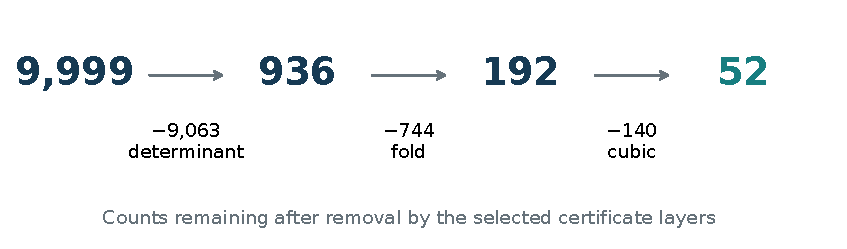
\includegraphics[width=\linewidth]{obstruction_partition.pdf}
\caption{Removal of mechanism classes by successive certificate layers. The intermediate numbers count classes not yet decided by the preceding schemes; they do not assert that every remaining class realizes the preceding degeneracy conditions. The label of a class names the certificate that decides it, not the first jet condition the network can satisfy.}
\label{fig:partition}
\end{figure}

\section{Exact positive templates}\label{sec:positive}

Each of the 52 positive records supplies an equilibrium at $x^*=\one$, positive rates, vectors $p,q,h$ and a selected pair of rate indices $(i,j)$. Every entry is a polynomial with rational coefficients in a real root $t$ of a rational polynomial $m(t)$, together with a rational isolating interval for the root. Sixteen records are rational: they use $m(t)=t$ and $t=0$. Fifteen use a quadratic $m$ and twenty-one a cubic $m$. The Lean proofs establish the algebraic certificate $\AlgCusp$ for each record: the equilibrium equations, all identities in~\eqref{eq:jet}, positivity of the state and rates, nonzero trace, nonzero cubic contraction and the raw rank condition~\eqref{eq:raw}.

For the analytic conclusion we additionally need the corrected minor~\eqref{eq:corrected}. At unit state, with $e_r$ the $r$-th coordinate direction in rate space,
\[
 \alpha_r=pN_r=p\,f_k(e_r),\qquad \eta_r=pN_r\,(a_r\!\cdot\!q)=p\,J_k(e_r)\,q,
\]
and the trace-scaled corrected minor of the selected pair is
\begin{equation}\label{eq:D}
 D_{ij}=\alpha_i\bigl(\tau\eta_j-pB(q,N_j)\bigr)-\alpha_j\bigl(\tau\eta_i-pB(q,N_i)\bigr)
 =\tau\cdot\det\begin{pmatrix}a(e_i)&a(e_j)\\ b(e_i)&b(e_j)\end{pmatrix}.
\end{equation}
All quantities are reduced modulo $m$. Each record contains polynomials $U,V\in\Q[t]$ with
\begin{equation}\label{eq:bezout}
 U(t)\,D_{ij}(t)+V(t)\,m(t)=1
\end{equation}
identically in $\Q[t]$. At the chosen root of $m$ this gives $D_{ij}\ne0$, and since $\tau\ne0$ the corrected determinant $D_{ij}/\tau$ is nonzero. The trace-scaled form of the minor and its relation to the corrected matrix are the content of the Lean file \lean{ReducedUnfolding.lean}, which proves the generic identity behind~\eqref{eq:D} for any certificate with nonzero trace.

\begin{proposition}[Positive existence]\label{prop:positive}
Every representative in Table~\ref{tab:all} admits an ordinary transverse cusp at positive concentrations and positive rates.
\end{proposition}
\begin{proof}
For each of the 52 records the exact checker verifies, by rational polynomial arithmetic modulo $m$ and exact root isolation, that $t$ is a root of $m$ in the stated interval, that the state and rates are positive, that the equilibrium and all jet identities~\eqref{eq:jet} hold, that $\tau\ne0$ and $c\ne0$, and that~\eqref{eq:bezout} holds identically for the recomputed $D_{ij}$. The record payloads agree with the Lean source files and their bound hashes. Hence every record satisfies the hypotheses of Proposition~\ref{prop:analytic} for its selected pair. No floating-point tolerance enters any existence or nonvanishing test.
\end{proof}

The 52 B\'ezout identities and root data are part of the machine-readable supplement, and the check script accompanying the paper re-verifies every identity~\eqref{eq:bezout} symbolically. They are compact exact evidence for the analytic correction; we do not describe them as 52 additional Lean analytic theorems.

In all 52 records the signs are the same: $\tau<0$, $c<0$ and $D_{ij}>0$, proved by exact rational interval arithmetic on the isolating interval. The sign of $\tau$ and $c$ is used in Section~\ref{sec:consequences}.

\subsection{A rational representative}\label{sec:example}
Template 02 makes the positive argument fully explicit:
\begin{equation}\label{eq:example}
 0\to X,\qquad X\to0,\qquad Y\to2X,\qquad 2X\to X+Y,\qquad X+Y\to Y,
\end{equation}
with rates $(k_1,\dots,k_5)=(1,3,3,3,1)/11$ and vector field
\begin{equation}\label{eq:examplefield}
 \dot x=k_1-k_2x+2k_3y-k_4x^2-k_5xy,\qquad \dot y=k_4x^2-k_3y .
\end{equation}
At $x^*=(1,1)$ one may take
\[
 J=\frac1{11}\begin{pmatrix}-10&5\\6&-3\end{pmatrix},\qquad
 q=\frac1{11}\binom{5}{10},\qquad
 p=\Bigl(\frac{33}{65},\frac{11}{13}\Bigr),\qquad
 h=\frac1{1573}\binom{-250}{150},
\]
and direct substitution gives
\[
 \tau=-\frac{13}{11},\qquad c=-\frac{75}{17303},\qquad D_{1,5}=\frac{27}{65},
\]
so the corrected determinant for the pair $(k_1,k_5)$ is $D_{1,5}/\tau=-297/845$, and $U=65/27$, $V=0$ certify~\eqref{eq:bezout}.

The same network admits a direct scalar reduction that displays the cusp without any local theory. Keep $k_3=k_4=3/11$ and $k_5=1/11$ and write $a=k_1$, $b=k_2$. The second equilibrium equation gives $y=x^2$, and substituting into the first, with
\[
 x=1+z,\qquad a=\frac{1+\mu-\nu}{11},\qquad b=\frac{3-\nu}{11},
\]
yields exactly
\begin{equation}\label{eq:cubicexample}
 11\,\dot x\big|_{y=x^2}=\mu+\nu z-z^{3}.
\end{equation}
The map $(\mu,\nu)\mapsto(a,b)$ is affine and invertible, the base rates are positive, and~\eqref{eq:cubicexample} is the universal unfolding of the cusp singularity. The fold curve is $(\mu,\nu)=(-2z^3,3z^2)$, and the region $27\mu^2<4\nu^3$ contains three positive equilibria (Figure~\ref{fig:example}). This is a regular cusp unfolding by the pair $(k_1,k_2)$, a different admissible pair from the certified $(k_1,k_5)$.

\begin{figure}[tb]
\centering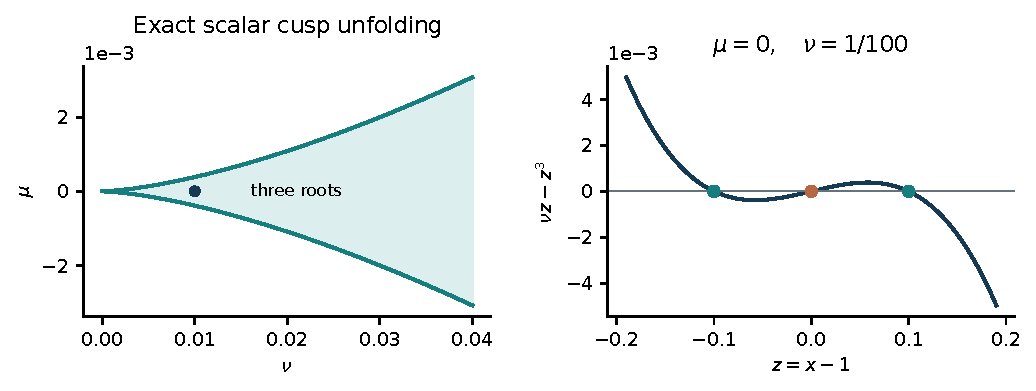
\includegraphics[width=\linewidth]{rational_cusp.pdf}
\caption{Exact equilibrium reduction of template 02, equation~\eqref{eq:cubicexample}. Left: the fold curve $(\mu,\nu)=(-2z^3,3z^2)$ bounds the three-root region. Right: at the marked parameter value $\mu=0$, $\nu=1/100$ the roots are $z=-1/10,0,1/10$, all corresponding to positive concentrations. The plots illustrate an exact polynomial identity, not fitted continuation data.}
\label{fig:example}
\end{figure}

\section{Exhaustive coverage and proof of the main theorem}\label{sec:coverage}

\subsection{The formal statement}
The Lean development represents a literal network as a structure with five reactant and five product complexes, injective reaction pairs and no self-reactions, and the model as the predicate \lean{IsPlanarBimolecular252}. The algebraic certificate $\AlgCusp$ is the predicate \lean{AdmitsTransverseCusp}. The following listing reproduces the definition of a valid certificate, with the network's mass-action field, Jacobian, Hessian and their rate derivatives as defined functions.

\begin{lstlisting}
structure CuspCertificate {m : ℕ} (Q : SmallPlanarNetwork m) where
  state : Species → ℝ
  rates : Fin m → ℝ
  rightKernel : Species → ℝ
  leftKernel : Species → ℝ
  centerCorrection : Species → ℝ
  unfoldingDirections : Fin 2 → Fin m → ℝ
\end{lstlisting}

A certificate is valid when its state and rates are positive, the state is an equilibrium, the stored vectors satisfy the jet system~\eqref{eq:jet} with nonzero trace and nonzero mixed cubic contraction, and the raw unfolding matrix on the two stored directions is nonsingular:

\begin{lstlisting}
def CuspCertificate.Valid (C : CuspCertificate Q) : Prop :=
  PositiveVector C.state ∧ PositiveVector C.rates ∧
  (∀ i, Q.massAction C.rates C.state i = 0) ∧
  (∀ i, Q.jacobianApply C.rates C.state C.rightKernel i = 0) ∧
  (∀ j, ∑ i : Species, C.leftKernel i * Q.jacobian C.rates C.state i j = 0) ∧
  dot C.leftKernel C.rightKernel = 1 ∧
  Q.jacobian C.rates C.state 0 0 + Q.jacobian C.rates C.state 1 1 ≠ 0 ∧
  dot C.leftKernel (Q.hessianApply C.rates C.state C.rightKernel C.rightKernel) = 0 ∧
  (∀ i, Q.jacobianApply C.rates C.state C.centerCorrection i =
      -Q.hessianApply C.rates C.state C.rightKernel C.rightKernel i) ∧
  dot C.leftKernel C.centerCorrection = 0 ∧
  dot C.leftKernel
      (Q.hessianApply C.rates C.state C.rightKernel C.centerCorrection) ≠ 0 ∧
  Matrix.det C.unfoldingMatrix ≠ 0

def AdmitsTransverseCusp (Q : SmallPlanarNetwork m) : Prop :=
  ∃ C : CuspCertificate Q, C.Valid
\end{lstlisting}

Here \lean{unfoldingMatrix} is the raw matrix~\eqref{eq:raw} evaluated on the two stored directions. The public theorem and its negative direction are unconditional:

\begin{lstlisting}
theorem no_cusp_if_not_in_52 (Q : SmallPlanarNetwork 5)
    (hQ : IsPlanarBimolecular252 Q)
    (hnot : ¬ BelongsToBimolecularCuspClass Q) : ¬ AdmitsTransverseCusp Q

theorem classify_planar_bimolecular_2_5_2_cusps
    (Q : SmallPlanarNetwork 5) (hQ : IsPlanarBimolecular252 Q) :
    AdmitsTransverseCusp Q ↔ BelongsToBimolecularCuspClass Q
\end{lstlisting}

Membership \lean{BelongsToBimolecularCuspClass Q} means that the literal network $Q$ has an exact coded realization whose source-lookup record is valid and carries the positive tag; such a record names the positive template, the reaction matching and the species orientation that connect $Q$ to it. It is source-faithful: no representative is silently identified with a network, and every step is witnessed by exact reaction-set equality, species exchange or positive column scaling, each of which is proved to preserve and reflect \lean{AdmitsTransverseCusp}.

\subsection{Structure of the formal proof}
The formal proof has the following layers; every layer is a separate Lean module (Table~\ref{tab:formal}).
\begin{enumerate}[label=\textup{(\arabic*)}]
\item \emph{Necessary structure.} From a valid certificate the development derives the structural conditions of Section~\ref{sec:reductions}: rank two, a strictly positive kernel vector, and at least four reactant complexes. These define the eligible catalogue of $60{,}036$ literal reaction sets.
\item \emph{Mechanism partition.} Four lists of mechanism representatives, of lengths $52$, $9{,}063$, $744$ and $140$, carry positive certificates or obstruction certificates checked instance by instance. The four outcome tags are proved exhaustive and pairwise exclusive, and $52+9063+744+140=9999$ is a theorem.
\item \emph{Source records.} $30{,}051$ records, one per species-exchange orbit of $\Eligible$, each contain a literal source, the index of its mechanism representative, matching and orientation data and the outcome tag. Docking (positive simple equivalence of the source to the oriented representative, proved semantically from a division-free integer ray check) and target consistency (agreement of the tag with the layer) are checked separately and combined into record validity.
\item \emph{Lookup.} A table of $60{,}036$ oriented source keys maps every eligible set to a record index and an orientation flag. The lookup is proved complete (every eligible set has an entry) and sound (every entry is eligible), and key injectivity converts key equality into exact equality of reaction sets.
\item \emph{Transport.} A valid record transports its outcome to its literal source: positive records yield \lean{AdmitsTransverseCusp}, obstruction records yield its negation, along the proved equivalence transports.
\end{enumerate}

The size of the certificate payloads made a naive coverage proof impractical, and the solution is a reusable proof-engineering idea. The coverage argument never elaborates the large algebraic records while it reasons about the lookup table. Instead, sixty-one bounded Lean batch proofs establish that mapping the actual records, in their stored order, to their pair of compact keys reproduces a packed key list; list-map and concatenation identities assemble the batches; a generic indexed-lookup lemma then recovers the actual record for any key; and key injectivity supplies the reaction-set equality. Numerical preflights guided the representation, but the key/record equalities and the coverage implication are Lean theorems.

\subsection{Proof of Theorem~\ref{thm:main}}
\begin{proof}
Suppose first that $Q$ admits an ordinary transverse cusp. Lemma~\ref{lem:necessary} gives $\AlgCusp(Q)$, so by \lean{classify_planar_bimolecular_2_5_2_cusps} the literal network $Q$ is source-faithfully covered by a positive record. Unwinding the record, $Q$ is simply equivalent up to species exchange to one of the 52 representatives, and by Lemma~\ref{lem:key} its key is that representative's key. (Equivalently, and without appeal to the analytic level: were $Q$'s record an obstruction record, the corresponding scheme of Section~\ref{sec:negative} would contradict a necessary state-jet condition of the cusp.)

Conversely, if $K(Q)$ equals a listed key, Lemma~\ref{lem:key} makes $Q$ simply equivalent up to species exchange to the representative, Proposition~\ref{prop:positive} gives that representative an ordinary transverse cusp, and reaction permutation, positive rate reparameterization and species exchange transport the cusp, together with its transverse unfolding by the corresponding pair of rates, to $Q$.

The 52 listed keys are pairwise distinct by exact finite comparison, so the representatives are pairwise inequivalent by Lemma~\ref{lem:key}.
\end{proof}

\section{Consequences}\label{sec:consequences}

\subsection{Five distinct reactants}
\begin{proof}[Proof of Corollary~\ref{cor:five-sources}]
All 52 representatives have five distinct reactant complexes (Table~\ref{tab:all}), and the number of distinct reactants is invariant under Definition~\ref{def:equiv}. Table~\ref{tab:counts} shows that the $8{,}000$ mechanism classes with four reactants are all decided by obstructions. Thus the general bound of Lemma~\ref{lem:four} is not sharp in this five-reaction class: four sources are necessary in general, but five are necessary here.
\end{proof}

The Lean development exports the general lower bound (\lean{four_reactants_necessary_for_bimolecular_cusp}) and the existence of a five-reactant witness (\lean{five_distinct_reactants_suffice}); the sharpened statement of Corollary~\ref{cor:five-sources} is read off from the exact partition, which is verified by the check script, and is not a separate Lean export.

\subsection{Reaction minimality}
\begin{proof}[Proof of Corollary~\ref{cor:minimal}]
Banaji, Boros and Hofbauer proved that no full-rank planar quadratic mass-action network with four reactions admits a cusp unfolded by its rate constants~\citep[Theorem~36]{BBH2024}; this covers the rank-two planar bimolecular networks with four reactions. With at most three reactions there are at most three sources, and Lemma~\ref{lem:four} applies. Rank-one planar quadratic systems have a one-dimensional stoichiometric class on which the equilibrium equation is a polynomial of degree at most two, so they have at most two isolated positive equilibria and no cubic degeneracy; rank zero is trivial. Template 02 with five bimolecular reactions attains the bound, so five reactions is the minimum and each of the 52 classes realizes it.
\end{proof}

\subsection{Every class organizes bistability}
Recall that in all 52 records $\tau<0$ and $c<0$.

\begin{proof}[Proof of Corollary~\ref{cor:bistable}]
Fix a representative and its certified pair $(k_i,k_j)$. By Proposition~\ref{prop:analytic} the reduced equation $g(z,k)=0$ is a versal unfolding of $z\mapsto cz^3$ with $c<0$, so for rates in the interior of the cusp region, close to $k^*$, $g(\cdot,k)$ has three simple zeros $z_1<z_2<z_3$ with $g_z(z_1,k)<0$, $g_z(z_2,k)>0$, $g_z(z_3,k)<0$. Let $x(z,k)=x^*+zq+y(z,k)$ be the corresponding equilibria and $J(z,k)$ their Jacobians. Differentiating the identity $f(x(z,k),k)=q\,g(z,k)$ in $z$ gives $J(z,k)\,(q+y_z)=g_z\,q$. Writing $J(z,k)$ in the basis $\{q+y_z,\,w\}$ with $w$ spanning $\Ker p$, its matrix has first column $(g_z,-g_z\gamma)^{\T}$ where $y_z=\gamma w$, and second column $(\ast,\beta)^{\T}$ with $\beta=\tau$ and $\gamma=0$ at the cusp point; hence $\det J(z,k)=g_z\,(\beta+\gamma\,\ast)$, whose second factor is close to $\tau<0$ near the cusp. So $\det J<0$ at the middle zero and $\det J>0$ at the outer zeros, while $\tr J$ is close to $\tau<0$ at all three. The outer equilibria are asymptotically stable, the middle one is a saddle, and all three are positive because $x^*$ is positive.
\end{proof}

The mechanism is an exact rational instance for template 02. With $0<\varepsilon<1$ take $k_1=(1-\varepsilon^2)/11$, $k_2=(3-\varepsilon^2)/11$ and $k_3,k_4,k_5$ as in~\eqref{eq:example}. Then $\mu=0$, $\nu=\varepsilon^2$ in~\eqref{eq:cubicexample}, the three equilibria are $x=1-\varepsilon,1,1+\varepsilon$ with $y=x^2$, and their Jacobians have
\[
 \det J=\frac{6\varepsilon^2}{121},\quad -\frac{3\varepsilon^2}{121},\quad \frac{6\varepsilon^2}{121},\qquad
 \tr J=\frac{8\varepsilon-13}{11},\quad \frac{\varepsilon^2-13}{11},\quad -\frac{8\varepsilon+13}{11},
\]
respectively: a stable node, a saddle and a stable node. At $\varepsilon=1/10$ the rates are $(99/1100,\,299/1100,\,3/11,\,3/11,\,1/11)$ and the equilibria $(9/10,81/100)$, $(1,1)$, $(11/10,121/100)$ have determinants $3/6050$, $-3/12100$, $3/6050$ and traces $-61/55$, $-1299/1100$, $-69/55$. These identities are verified symbolically by the check script. Corollary~\ref{cor:bistable} is an existential local statement for each class; it describes neither all cusp points nor the global parameter space of the class.

\subsection{Ray geometry does not determine cusp existence}\label{sec:rays}
A natural conjecture is that cusp existence depends only on the unlabelled geometry of the five stoichiometric rays, or at least on their oriented matroid. The classification refutes it. The 52 positive classes realize 31 distinct unlabelled multisets of primitive directed rays and only five distinct rank-two oriented matroids, so the reactant labels carry most of the information. The lexicographically smallest collision between a positive and a negative class is
\begin{align*}
 \text{positive (template 00):}&\quad 0\to X,\ X\to0,\ Y\to2X,\ 2X\to X+Y,\ X+Y\to0;\\
 \text{negative (cubic layer):}&\quad 0\to X,\ X\to0,\ Y\to2X,\ X+Y\to0,\ X+Y\to2Y .
\end{align*}
The reactions $2X\to X+Y$ and $X+Y\to2Y$ both have stoichiometric vector $(-1,1)$, so the two networks have the same five directed vectors, not merely the same matroid; they differ only in the reactant of that one reaction, and the negative network has four distinct reactants.

The reason is explicit. Write the rates of the negative network, in the displayed order, as $a,b,d,e,f$. Its vector field is
\[
 \dot x=a-bx+2dy-(e+f)xy,\qquad \dot y=\bigl((f-e)x-d\bigr)\,y .
\]
A positive equilibrium requires $f>e$ and $x=d/(f-e)$, and there $\det J=-d(f-3e)y$. A singular positive equilibrium therefore requires $f=3e$, hence $x=d/(2e)$, and then the first equation reads $a-bd/(2e)=0$ independently of $y$: the singular equilibrium lies on a whole line of equilibria. The degeneracy is a continuum, never an isolated cubic cusp, and the cubic-degeneracy certificate of Section~\ref{sec:negative} is its exact witness. The same ray geometry supports different nonlinear equilibrium geometry because the reactant label changed. A complete reactant-labelled key is the invariant of Lemma~\ref{lem:key}, and it yields the finite classification itself; we assert no smaller structural generator theorem.

\begin{figure}[tb]
\centering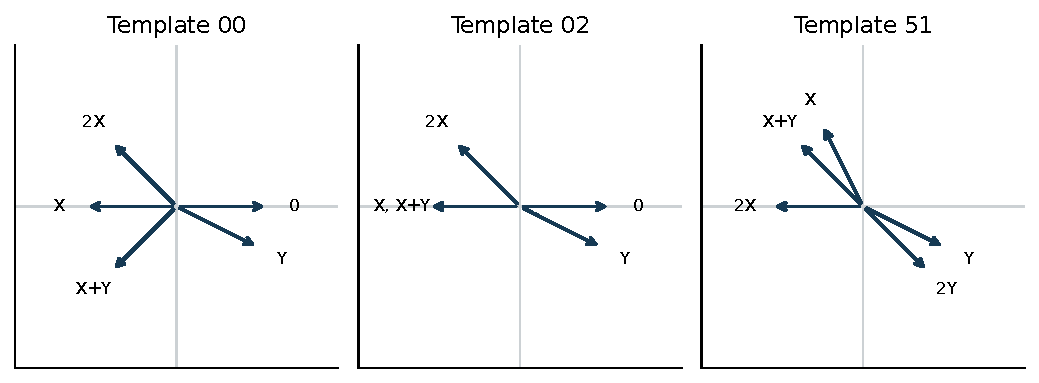
\includegraphics[width=.9\linewidth]{positive_rays.pdf}
\caption{Stoichiometric vectors of three positive templates, each arrow labelled by the reactant complex of its reaction. Templates 00 and 02 share four reactions and differ only in the product of the reaction with reactant $X+Y$. In template 02 the reactions $X\to0$ and $X+Y\to Y$ have the same vector $(-1,0)$, so its five reactions span only four rays; the reactant labels are what distinguish coincident rays, and Section~\ref{sec:rays} shows that they also decide cusp existence. Template 51 has five distinct rays and no reaction with reactant $0$.}
\label{fig:rays}
\end{figure}

\subsection{Inheritance}
Once analytic rate transversality is established, the inheritance theorem of Banaji, Boros and Hofbauer~\citep[Theorem~3.2]{BBH2025} applies: every network in the 52 classes passes its nondegenerate cusp, with its transverse unfolding, to any enlargement obtained by the operations listed there, including rank-preserving addition of reactions, addition of inflow and outflow reactions, and the specified new-species constructions, and to any finite composition of such operations. This gives infinitely many larger mass-action networks, bimolecular or not, with certified cusps and the bistability of Corollary~\ref{cor:bistable}; the rank hypotheses on added reversible reactions and reaction splittings are essential, and arbitrary supernetworks are not covered. This is an application of a published theorem, not a new formal result.

\section{Verification and reproducibility}\label{sec:verification}

\subsection{Formal interfaces}
The reusable proof sources are under \path{proofs/SmallCusp/} in the supplement. The positive templates and the three obstruction layers are separate modules rather than one generated monolith; Table~\ref{tab:formal} lists the critical interfaces.

\begin{table}[tb]
\centering\small
\caption{Critical formal interfaces, with paths relative to \texttt{proofs/SmallCusp/}.}
\label{tab:formal}
\begin{tabular}{p{.40\linewidth}p{.54\linewidth}}\toprule
Role & Source module\\\midrule
Literal model and algebraic cusp predicate & \texttt{Source/SourceClasses.lean}\\
Trace-free unit-state normalization & \texttt{Normalization/TraceFreeCertificate.lean}\\
Positive templates (52) & \texttt{Cusp/PositiveCuspLayer.lean}\\
Trace-scaled corrected minor identity & \texttt{Cusp/ReducedUnfolding.lean}\\
Determinant exclusions (9,063) & \texttt{Obstruction/ConicDeterminantLayer.lean}\\
Quadratic exclusions (744) & \texttt{Obstruction/CircuitFoldLayer.lean}\\
Cubic exclusions (140) & \texttt{Obstruction/CubicResidualLayer.lean}\\
Outcome exhaustiveness and partition count & \texttt{Classification/CoverageTypes.lean}\\
Eligible catalogue cardinality (60,036) & \texttt{Classification/SourceCatalogueCount.lean}\\
Unconditional literal coverage & \texttt{Classification/SourceCoverageLookup.lean}\\
Public iff and negative theorem & \texttt{Classification/BimolecularClassification.lean}\\
Exported corollaries and counts & \texttt{Classification/BimolecularCorollaries.lean}\\\bottomrule
\end{tabular}
\end{table}

\subsection{Trust boundary}
The public theorems were verified with Lean 4.30.0 and the frozen Mathlib manifest of the repository, with warnings treated as errors, no \lean{sorry}, and exit code zero; the receipt covers $1{,}072$ dependency modules. Each of the two public exports reports the standard axioms \lean{Classical.choice}, \lean{Quot.sound} and \lean{propext} together with $3{,}826$ generated \lean{native_decide} axioms, and no unexpected axiom. Thus the finite computations (certificate checks, list lengths, key comparisons) trust Lean's compiled native-evaluation bridge, in addition to the Lean kernel and the frozen environment; this is not a claim of kernel-only reduction of every finite computation. The strict receipt records a $120.711$-second verification of the public module; this is provenance, not a benchmark of proof development or of a clean rebuild, which materializes the dependency modules first.

\subsection{What is formal and what is conventional}
\begin{itemize}
\item \emph{Lean theorems:} the model and certificate definitions; the necessary structural conditions for $\AlgCusp$, including the four-reactant bound; the soundness lemmas and all instances of the three obstruction schemes; the 52 positive $\AlgCusp$ certificates; exhaustiveness and exclusivity of the outcomes and the count $9{,}999$; the cardinalities $60{,}036$ and $30{,}051$; completeness and soundness of the lookup; the equivalence transports; the trace-scaled minor identity; and the unconditional public iff and negative theorem.
\item \emph{Conventional proofs in this paper:} the Lyapunov--Schmidt reduction of Proposition~\ref{prop:analytic}; Lemma~\ref{lem:necessary}; Lemma~\ref{lem:surround}; Lemma~\ref{lem:four} via~\citep{BF2026}; the key invariant, Lemma~\ref{lem:key}; the sign argument of Corollary~\ref{cor:bistable}; the continuum-degeneracy computation of Section~\ref{sec:rays}; the reduction to published results in Corollary~\ref{cor:minimal} and the inheritance remark.
\item \emph{Exact computer algebra, reproducible from the supplement:} the 52 corrected-minor B\'ezout identities and sign certificates; the independent enumeration of the $142{,}506$ literal sets and the counts $60{,}036$, $30{,}051$, $9{,}999$; pairwise distinctness of the 9,999 keys and of the 52 positive keys; the split of Table~\ref{tab:counts} by source count; the ray-skeleton and oriented-matroid counts of Section~\ref{sec:rays}; and the rational examples of Sections~\ref{sec:example} and~\ref{sec:consequences}.
\end{itemize}
Exporting the conventional steps as Lean declarations is a separate formalization project and is not claimed here.

\subsection{Supplement and check script}
The supplement contains the exact positive root and witness data, all corrected-minor B\'ezout certificates, the four representative partitions, the critical Lean dependency sources with SHA-256 hashes, the strict verification receipt, deterministic generators for the tables and figures, and reproduction instructions. The check script distributed with this paper re-derives, with SymPy, every number printed in the text: the enumeration counts, the partition and its source split, the degree distribution of the root polynomials, the 52 B\'ezout identities, the jet data and corrected minor of template 02, the scalar reduction~\eqref{eq:cubicexample}, the three-equilibria family and its rational instance, the collision computation of Section~\ref{sec:rays}, the receipt figures quoted above, and the rows of Table~\ref{tab:all} against the Lean records. The full positive catalogue can therefore be read without software, and its exact witnesses checked mechanically. The pinned Lean and Mathlib environment is a prerequisite for replaying the formal proof; it is not replaced by current dependencies.

\section{Discussion and open problems}\label{sec:discussion}

The classification settles the smallest planar bimolecular case of a cusp unfolded by rate constants, and it does so with the identity of every literal network preserved through the proof. Several questions are left open by design.

\emph{Comparison with the dual-equation approach.} Banaji's correspondence between original and dual fold and cusp conditions~\citep{B2026} is a different route to the same class, and Section~6.3 of that preprint announces a classification. When that list is available, a class-by-class comparison via the keys of Appendix~\ref{app:list} would be a valuable cross-check of two independent methods; we have not performed one, and our correctness does not depend on the dual-equation correspondence.

\emph{Larger models.} The same pipeline applies to five-reaction networks with trimolecular products, to more reactions, and to three species, with the enumeration and certificate counts growing accordingly. The $(2,5,2)$ trimolecular-product class is defined in the Lean development but not classified here. The separate problem of four-reaction planar networks with multiple nonnegative stable equilibria on the boundary of the orthant is also outside this theorem.

\emph{Coarser equivalences.} Our count is under Definition~\ref{def:equiv}. Under dynamical equivalence, or under diagonal equivalence that also rescales rows of $N$, several of the 52 classes may merge; determining the coarser count is a distinct problem.

\emph{The negative categories are not strata.} The obstruction that decides a class is the first sufficient certificate found in a fixed order; it does not assert that the class realizes the preceding degeneracies. A classification of the negative classes by the strongest jet condition they can realize (nonsingular everywhere, folds only, degenerate folds only) is a natural refinement.

\emph{Formalization of the analytic bridge.} The implicit-function reduction of Proposition~\ref{prop:analytic} and the corrected-minor instances are within reach of Mathlib's analysis library, and formalizing them would move Theorem~\ref{thm:main} entirely inside the formal core.

\emph{Global dynamics.} Corollary~\ref{cor:bistable} is local. Which of the 52 classes admit globally attracting bistability, and which combine the cusp with Hopf or Bogdanov--Takens points, are questions for the methods of~\citep{BBH2024,BB2023}.

\bibliographystyle{plainnat}
\bibliography{refs}

\clearpage
\appendix
\section{Complete list of positive representatives}\label{app:list}
Table~\ref{tab:all} lists the 52 pairwise inequivalent cusp-admitting classes. The five reactions of each row are ordered as in its exact witness; row identifiers are zero-based and match the ordinals of the supplement. Column $d$ is the degree of the witness root polynomial $m$ ($d=1$ means a rational witness with $m(t)=t$; the degree is not an assertion of irreducibility), and $(i,j)$ is the one-based pair of rate indices whose corrected minor is certified by~\eqref{eq:bezout}. The symbol $0$ denotes the empty complex. All rows have five distinct reactant complexes. The key of a row is recovered directly by~\eqref{eq:key}, and equivalence is exactly Definition~\ref{def:equiv}. The rational example~\eqref{eq:example} is row 02.

\begingroup\small
\setlength{\tabcolsep}{4pt}
\renewcommand{\arraystretch}{1.12}
\begin{longtable}{rlllllrr}
\caption{The 52 pairwise inequivalent cusp-admitting classes.}\label{tab:all}\\
\toprule
ID & Reaction 1 & Reaction 2 & Reaction 3 & Reaction 4 & Reaction 5 & $d$ & $(i,j)$\\\midrule
\endfirsthead
\multicolumn{8}{l}{\small Table~\thetable\ continued}\\
\toprule
ID & Reaction 1 & Reaction 2 & Reaction 3 & Reaction 4 & Reaction 5 & $d$ & $(i,j)$\\\midrule
\endhead
\midrule\multicolumn{8}{r}{\small Continued on the next page}\\\endfoot
\bottomrule\endlastfoot
00 & $0\to X$ & $X\to 0$ & $Y\to 2X$ & $2X\to X{+}Y$ & $X{+}Y\to 0$ & 3 & 1,5 \\
01 & $0\to X$ & $X\to 0$ & $Y\to 2X$ & $2X\to X{+}Y$ & $X{+}Y\to X$ & 3 & 1,5 \\
02 & $0\to X$ & $X\to 0$ & $Y\to 2X$ & $2X\to X{+}Y$ & $X{+}Y\to Y$ & 1 & 1,5 \\
03 & $0\to X$ & $X\to 0$ & $Y\to 2X$ & $2X\to X{+}Y$ & $2Y\to X$ & 3 & 1,5 \\
04 & $0\to X$ & $X\to 0$ & $Y\to 2X$ & $2X\to X{+}Y$ & $2Y\to 0$ & 3 & 1,5 \\
05 & $0\to X$ & $X\to Y$ & $Y\to 2Y$ & $X{+}Y\to 0$ & $2Y\to X$ & 3 & 2,5 \\
06 & $0\to X$ & $X\to Y$ & $Y\to 2Y$ & $X{+}Y\to 0$ & $2Y\to 0$ & 3 & 2,5 \\
07 & $0\to X$ & $X\to Y$ & $Y\to 2Y$ & $X{+}Y\to 0$ & $2Y\to 2X$ & 2 & 2,5 \\
08 & $0\to X$ & $X\to X{+}Y$ & $Y\to 2Y$ & $X{+}Y\to 0$ & $2Y\to X$ & 1 & 2,5 \\
09 & $0\to X$ & $X\to X{+}Y$ & $Y\to 2Y$ & $X{+}Y\to 0$ & $2Y\to 0$ & 1 & 2,5 \\
10 & $0\to X$ & $X\to X{+}Y$ & $Y\to 2Y$ & $X{+}Y\to 0$ & $2Y\to 2X$ & 1 & 2,5 \\
11 & $0\to X$ & $X\to 2Y$ & $Y\to 0$ & $2X\to 0$ & $X{+}Y\to 2X$ & 1 & 1,4 \\
12 & $0\to X$ & $X\to 2Y$ & $Y\to 0$ & $2X\to 0$ & $2Y\to 2X$ & 3 & 1,4 \\
13 & $0\to X$ & $X\to 2Y$ & $2X\to 0$ & $X{+}Y\to 2X$ & $2Y\to 0$ & 3 & 1,3 \\
14 & $0\to X$ & $X\to 2Y$ & $Y\to 0$ & $2X\to Y$ & $X{+}Y\to 2X$ & 3 & 1,4 \\
15 & $0\to X$ & $X\to 2Y$ & $Y\to 0$ & $2X\to Y$ & $2Y\to 2X$ & 2 & 1,4 \\
16 & $0\to X$ & $X\to 2Y$ & $2X\to Y$ & $X{+}Y\to 2X$ & $2Y\to 0$ & 2 & 1,3 \\
17 & $0\to X$ & $X\to 2Y$ & $2X\to X{+}Y$ & $X{+}Y\to 2X$ & $2Y\to 0$ & 3 & 1,3 \\
18 & $0\to X$ & $X\to 2Y$ & $Y\to 0$ & $X{+}Y\to 0$ & $2Y\to 2X$ & 2 & 1,4 \\
19 & $0\to X$ & $X\to 2Y$ & $Y\to 0$ & $X{+}Y\to X$ & $2Y\to 2X$ & 1 & 1,4 \\
20 & $0\to X$ & $X\to 2Y$ & $Y\to 0$ & $X{+}Y\to Y$ & $2Y\to 2X$ & 2 & 1,4 \\
21 & $0\to X$ & $X\to 2Y$ & $Y\to 2Y$ & $X{+}Y\to 0$ & $2Y\to X$ & 2 & 2,5 \\
22 & $0\to X$ & $X\to 2Y$ & $Y\to 2Y$ & $X{+}Y\to 0$ & $2Y\to 0$ & 3 & 2,5 \\
23 & $0\to X$ & $X\to 2Y$ & $Y\to 2Y$ & $X{+}Y\to 0$ & $2Y\to 2X$ & 2 & 2,5 \\
24 & $0\to X$ & $Y\to 2Y$ & $2X\to Y$ & $X{+}Y\to 0$ & $2Y\to X$ & 1 & 3,5 \\
25 & $0\to X$ & $Y\to 2Y$ & $2X\to Y$ & $X{+}Y\to 0$ & $2Y\to 0$ & 3 & 3,5 \\
26 & $0\to X$ & $Y\to 2Y$ & $2X\to Y$ & $X{+}Y\to 0$ & $2Y\to 2X$ & 2 & 3,5 \\
27 & $0\to X$ & $Y\to 2Y$ & $2X\to X{+}Y$ & $X{+}Y\to 0$ & $2Y\to X$ & 2 & 3,5 \\
28 & $0\to X$ & $Y\to 2Y$ & $2X\to X{+}Y$ & $X{+}Y\to 0$ & $2Y\to 0$ & 3 & 3,5 \\
29 & $0\to X$ & $Y\to 2Y$ & $2X\to X{+}Y$ & $X{+}Y\to 0$ & $2Y\to 2X$ & 3 & 3,5 \\
30 & $0\to X{+}Y$ & $X\to 0$ & $Y\to 2X$ & $2X\to X{+}Y$ & $X{+}Y\to 0$ & 2 & 1,5 \\
31 & $0\to X{+}Y$ & $X\to 0$ & $Y\to 2X$ & $2X\to X{+}Y$ & $X{+}Y\to X$ & 3 & 1,5 \\
32 & $0\to X{+}Y$ & $X\to 0$ & $Y\to 2X$ & $2X\to X{+}Y$ & $X{+}Y\to Y$ & 1 & 1,5 \\
33 & $0\to X{+}Y$ & $X\to 0$ & $Y\to 2X$ & $2X\to X{+}Y$ & $2Y\to X$ & 1 & 1,5 \\
34 & $0\to X{+}Y$ & $X\to 0$ & $Y\to 2X$ & $2X\to X{+}Y$ & $2Y\to 0$ & 2 & 1,5 \\
35 & $0\to X{+}Y$ & $X\to 0$ & $Y\to 2X$ & $X{+}Y\to 2Y$ & $2Y\to X$ & 1 & 1,5 \\
36 & $0\to X{+}Y$ & $X\to 0$ & $Y\to 2X$ & $X{+}Y\to 2Y$ & $2Y\to 0$ & 3 & 1,5 \\
37 & $0\to X{+}Y$ & $X\to 2Y$ & $2X\to 0$ & $X{+}Y\to 2X$ & $2Y\to 0$ & 2 & 1,3 \\
38 & $0\to X{+}Y$ & $X\to 2Y$ & $2X\to Y$ & $X{+}Y\to 2X$ & $2Y\to 0$ & 1 & 1,3 \\
39 & $0\to X{+}Y$ & $X\to 2Y$ & $2X\to X{+}Y$ & $X{+}Y\to 2X$ & $2Y\to 0$ & 3 & 1,3 \\
40 & $X\to 2X$ & $Y\to 2Y$ & $2X\to Y$ & $X{+}Y\to 0$ & $2Y\to X$ & 1 & 3,5 \\
41 & $X\to 2X$ & $Y\to 2Y$ & $2X\to Y$ & $X{+}Y\to 0$ & $2Y\to 2X$ & 3 & 3,5 \\
42 & $X\to 2X$ & $Y\to 2Y$ & $2X\to X{+}Y$ & $X{+}Y\to 0$ & $2Y\to 2X$ & 1 & 3,5 \\
43 & $X\to Y$ & $Y\to 2X$ & $2X\to 0$ & $X{+}Y\to 2Y$ & $2Y\to X$ & 1 & 1,5 \\
44 & $X\to Y$ & $Y\to 2X$ & $2X\to 0$ & $X{+}Y\to 2Y$ & $2Y\to 0$ & 1 & 1,5 \\
45 & $X\to Y$ & $Y\to 2X$ & $2X\to 0$ & $X{+}Y\to 2Y$ & $2Y\to 2X$ & 1 & 1,5 \\
46 & $X\to X{+}Y$ & $Y\to 2X$ & $2X\to 0$ & $X{+}Y\to 2Y$ & $2Y\to X$ & 3 & 1,5 \\
47 & $X\to X{+}Y$ & $Y\to 2X$ & $2X\to 0$ & $X{+}Y\to 2Y$ & $2Y\to 0$ & 2 & 1,5 \\
48 & $X\to X{+}Y$ & $Y\to 2X$ & $2X\to 0$ & $X{+}Y\to 2Y$ & $2Y\to 2X$ & 3 & 1,5 \\
49 & $X\to 2Y$ & $Y\to 2X$ & $2X\to 0$ & $X{+}Y\to 2X$ & $2Y\to 0$ & 2 & 2,3 \\
50 & $X\to 2Y$ & $Y\to 2X$ & $2X\to 0$ & $X{+}Y\to 2Y$ & $2Y\to X$ & 2 & 1,5 \\
51 & $X\to 2Y$ & $Y\to 2X$ & $2X\to 0$ & $X{+}Y\to 2Y$ & $2Y\to 2X$ & 3 & 1,5 \\

\end{longtable}
\endgroup

\end{document}
